\setcounter{chapter}{ 26 }
\chapter{\textbf{``Terminus Rising'', part 1} }


\subChapterTitle{``It's All Just Psychosomatic''} 

\deets{Suko}{June 25th, 2014}



We're sent on an important diplomatic mission.  Someone's gonna get punched.






\jumpHeadline{SAC-09}

\sceneHeadline{Dr. Gerhauser's Office- Hayley and Dr. Gerhauser}

After stalking her all day, Hayley is finally informed by Swan that Dr. Gerhauser has a few minutes to talk.  Dr. Gerhauser's office is full of stuff. There is a \hl{circular table}\footnote{\textbf{Nathaniel Ford }Just to clarify; circled around her seat, console style. Or Colbert Report style \textsubscript{08/10/14 11:20pm}}, covered in stacks of books.  Shelves are full of things like microscopes, datapads and files.  There are neat stacks of clothing on the floor, everything from scrubs to nice clothing.  There appears to be an organizational system to all the items, but it is not easy to see what it is.  There is one chair not covered by books.



Dr. G is typing into a computer and doesn't look up as Hayley enters.  Hayley goes to stand next to the chair but does not sit down.  She politely waits for an acknowledgement.  And waits.  When it clear that Dr. G won't say anything, Hayley speaks, ``I would like to request access to the Cistern.''

``Why?''

``Because- because I need to be there?''

Dr. Gerhauser spins and looks at a file on another monitor.  ``Nothing in your record indicates a medical reason for it.''

``It's safer there.  Also it will relieve pain, since I do not want to take drugs.''

``Pain?''

``From my leg.''

``That's still persistent?''

``Yes.''

``Psychosomatic then.  So do you want something from me to make you feel better?''

``You are a doctor, isn't that what you do?'' asks Hayley, starting to feel worried.

``How many doctors have actually made you feel better?''  Dr. Gerhauser thinks about it for a moment and then says, ``Nevermind'' just as Hayley says ``Four.''

``Why should I help you?'' asks Dr. Gerhauser.

``Don't you want the team to do well?''

``And access to the Cistern will make the team do better?''

``It will help me protect them better.''

``That type of argument may work on my sister, but not on me.  Try asking her.''

``But I need medical clearance,'' says Hayley, very confused now.

``Oh right.  Tell me again why I should help you?''

``Why should I?  I'm making a request.''

``Oh.  Well then.  Request denied.''Hayley takes a long moment to absorb this information, staring at Dr. Gerhauser who has gone back to typing on the keyboard and ignoring Hayley.  Hayley notes that Dr. Gerhauser seems a little better, probably not on drugs any longer but she looks tired.  Hayley turns to go, then pauses.  After having some internal debate she says, ``I'm certain you know your health best, but you should get more rest.''

Dr. Gerhauser ignores her and says nothing.``It would make him sad to see you like this.''

Dr. Gerhauser misses a keystroke at that but doesn't look up and Hayley closes the door quietly behind her.



Hayley goes to Swan's desk and tells him, ``I would like to self-report that I am not fit for duty.''

Swan is alarmed and a bit flustered.  ``Ummm what exactly do you mean by that?''

``It is my self-assessment.  Is that not how I am supposed to make such a report?  I'm afraid I don't know the procedure for this yet.''

``Uh what is the reason?  Physical, emotional, psychological or some other reason?''

``What is psychosomatic?''

``Believing something that is not there.''

``That one.''

``I'll send for Dr. Gerhauser-''

``She's the one who told me.''

``Ah so you did get an assessment?''

``She told me I am psychosomatic, but nothing else.''

``So your symptoms are psychosomatic and you are self-reporting this?  Are you a danger to yourself or others?''

Hayley pauses for a long time.  Long enough that Swan gets nervous again.  ``I'm not certain.  That is why I am reporting myself,'' she finally replies.

``Can you elaborate?''

``I will not be performing at my best.''

``Hayley, just because you're not at your best doesn't mean that you are a danger to others.''

``But I am very upset and I don't seem to be able to get past it and it is very troubling to me.  I try to follow Agent Parvadi's orders to bottle it up and be angry but I don't want to be angry.  I don't like being angry.  So I cry a lot.''

``As your medical practitioner, I recommend letting it out.''

``But I can't do that out here.''

``Errrr....why?  Wait.  You know what, I understand.  We all have our safe places.''

``Really?  What's yours?'' asks Hayley curiously.

``Ah let's not talk about me right now.  Look, um.... let me see what I can do.''

``Thank you,'' Hayley smiles at him gratefully.

``Definitely let it out, even if you can't go to the Cistern.  And here, take these.  They are an anti-anxiety medication.''

``No thank you, I don't like drugs.''

``Yes but take them anyway.  Think of this as something like the medicines used to heal your body.  This will give your brain time to relax and heal itself.''

``Okay,'' says Hayley and takes the pills though she looks at them dubiously.  She looks back at Swan solemnly and tucks them away.   ``I trust you.''

``Good.  That's good.  Anything else?''

``Am I being manipulative?''

``What??''

``I asked you these things because I knew you might help and you are helping me.''

Swan blushes and flounders a little, ``Admittedly you have an odd BX and affect, but as your attending physician I, uh, have to understand that.''

``Why not Dr. Gerhauser?'' asks Hayley.

``What do you mean?''

``Why doesn't she have to understand that, understand us?''

``Well I mean she's a bit of an odd case...''

``She is?  She seems like a normal doctor.''

``She is, but she's not normal.''

``She seems normal to me.''

``What do you- nevermind.  So at this base, everyone wears the same uniform, right?  But we all have different skills.  Outwardly the same, but inwardly different.  Dr. Gerhauser, she's more of a scientist.''

``I don't understand the difference.''

``Generally a doctor is interested in recovery.  There are many types of doctors, like Trenton and Victors are called doctors but it's because they know a lot about something.  Scientists are more interested in the why of things.  They test things.''

``Yes, that is what I am familiar with.''

``Okay, maybe they are the same for you then.  Look, take the pills, they should help you get some sleep.''

Hayley nods.  She lingers and says, thinking hard, ``He- he told me to just ask for things I need.''

``Um, yes?''

``I don't think that Dr. Gerhauser is well.  Please look out after her.''

``I've been trying my best,'' says Swan solemnly.

Hayley smiles with relief and limps away.




\sceneHeadline{Morgan's Office- Jaya and Morgan}

Jari tells Jaya that Morgan has requested her presence.  Jaya is nervous.  Morgan is seated behind her desk.  There is a black box on her desk.  

``Agent Sir Ma'am Morgan Sir.  You asked me to report...?'' Jaya comes to rough attention.

``At ease,'' says Morgan.  Jaya sits awkwardly.

``There will be a mission briefing at 1400.  But there are some other tasks that I wish for you to perform.''

``Uh, I didn't bring my notebook,'' says Jaya.

``It is the duty of the commanding officer to return a soldier's effects to their family,'' says Morgan, pushing the box over to Jaya.  Jaya opens it.  Inside are the medals that she had salvaged from Oliver's things (Jaya takes a moment to be peeved at Jonah), and also a purple box and an arm band with the TA logo.

``Er- I'm a man down already and things are so busy- can't we utilize the postal service to deliver this?'' hedges Jaya.

``All cargo transport is disrupted currently, it is not feasible.  Additionally, you will already be there in Terminus with Oliver's father.''

``Oh.  Uh, this may not have been in the report- well it \textit{was} but not really.....may I speak freely?''

``Yes''

``His father was an ass.  He doesn't deserve it, any of this.''

``His father is a lynchpin on several committees that we need on our side.''

``Perhaps \textit{not} giving him the box would be better... He didn't really appreciate Oliver.''

``May I speak freely?'' asks Morgan.

``Yes,'' says Jaya nervously.

Morgan turns and sits back a little in a more relaxed posture.  ``How many \textit{not} horrible people have you met?''

``Well it's true, there are people who hardly impact you at all, and then there are people who do and you just want to, uh...'' Jaya mimes punching someone.

``So it is common.  Something you have dealt with before.  Can you deal with him without punching him in the face?''

``I believe in this, uh, situation, that I will delegate this responsibility to Jonah.''

``I feel like you have grown a lot as a commander,'' says Morgan.

``Yeah, I've done a lot to do the TA proud,'' brags Jaya and then looks at Morgan to see what she says about that.``Our cause would not be crippled if we lose Mr. Langdon.''

``I'll send Jonah, he'll handle it,'' says Jaya, sounding confident.

``You will have to be diplomatic at Terminus.  Many think that capitulation to the enemy is best.''

``So perhaps if my team and I make a strong showing...''

``You will be dealing with senators and former senators.  \hl{It is \textit{possible }you may be able to intimidate them.}\footnote{\textbf{Nathaniel Ford }I feel like there must have been an undertone of ``but it seems unlikely'' \textsubscript{07/03/14 10:43am}}\footnote{$\rightarrow$\textbf{Suko T }Yes the ``possible'' was stressed, I should probably italicize it. \textsubscript{07/03/14 12:00pm}}''

``How many Agents are there?''

``Several dozen, but none with your abilities.  The mission is to get Mr. Langdon on our side.''

``Who's side is that?  The TA?  The Directorate?  You?''

``You will be acting as my proxy.  So in this instance, yes, me.  You will need to convince him of the danger.  You have the best sense of what we're up against.''

``How about we just send the ones who want to capitulate to Octavius?''

``It won't work.''

``Who exactly do we have to talk to?'' asks Jaya.``Mr. Langdon, some members of the Triumvirate, and Agent Lorentz.''

``Our skill set will get this done,'' says Jaya and then rolls up the sleeve on her new mechanical arm.

``Don't hide it,'' says Morgan, indicating Jaya's new arm. ``But don't draw attention to it either.  It shows off the resources that you have available to you.  Be on the lookout for spies, Octavius certainly has agents in Terminus.  You are dismissed.''

Jaya gets up, without the box, and turns to leave.

Morgan clears her throat and Jaya turns back.  Morgan taps the box and Jaya takes it reluctantly.  Morgan has resumed her more formal posture and says, ``By the way, there has been some defacement of base property.  Please see that your team is informed that they are not to deface base property.  We have only the one elevator, it would be a shame to lose it.''

In the elevator, Jaya strokes the dent in the wall with a smile.




\sceneHeadline{Rook's lab- Jonah and Rook}

Jari tells Jonah that Rook would like to see him.  He gives him an unfamiliar room number, down in maintenance.  That area has been heavily remodeled and it takes a while for Jonah to get his bearings and find the room.  Inside the room, there are a variety of cylinders in different sizes and lots of machinery.  There are jars of green fluid and lots of devices lying on tables. The whole room smells of motor oil and slightly rancid milk.



Rook is wearing goggles and working on a mechanical arm.  ``Jonah, glad you could join me,'' he says without looking up as Jonah enters.  ``Come look at this.  I think you'll find this information valuable in the field.  Even though this is an older model it still should provide you with enough understanding to deal with Agent Parvadi's newer model.''  Jonah comes to stand next to Rook and Rook starts pointing at various sections of the arm. ``See these two parts?  They must be connected for power.''

``Ah, so not like a normal arm?'' asks Jonah.

``What do you mean by that?''

``The way that she was moving it, I thought that she could feel through it, but I don't see how...''

``There are receptors in her arm that provide feedback so that she can use it much like she would have used her original arm.''  Rook opens a panel. ``See this here, it is hollow for weight but this,'' Rook holds up a vial of green fluid, ``slots in here like this.  If the arm becomes damaged, pour this over the injury and it should help repair and seal the injury.  Be aware that it becomes highly exothermic.''

``Does the arm transmit pain?''

``She will be aware of damage to the arm, but it will not be painful.  Do keep in mind that this is a dangerous piece of equipment, treat it like a gun or an explosive.''

``There was a suggestions earlier that I may be able to influence the arm?''

``Agent Parvadi has a phrase to disengage the arm.''

``What is it?''

``You will have to ask her.  That may take some negotiation.  I would also ask that you encourage her not to put herself in the sort of situation that would require more modification.''

``Like...the portals?''

``Yes and other situations like that.  I am concerned that the lesson she has learned is that damage of that level is fixable.  And they can be, but it will change her.  I wouldn't recommend it as a life choice.''

``So you mean that there are limited supplies and she should not expect anything could be replaced?''

Rook gestures to the cylinders around them.  ``I could probably replace everything in her body but it would not be a preferable idea.''

``Best not to tell her that it's even a possibility then,'' says Jonah.

Rook continues to point out some of the inner workings of the arm and has Jonah practice with a few parts.

Rook asks, ``Another thing, consider if you want to be Hayley's Operator.''

``On our current path, I'll consider it,'' says Jonah.  ``Chief is reckless but doesn't want to die.  Hayley may have changed but I don't know how much.''

``Well it will take energy and time to set up the activation so you will need to plan a little ahead if you want to do it.''

``Are we going to be heading into danger?''

``If you asked Morgan, it is all dangerous.  Do you prefer statistics or calculus?''  at Jonah's puzzlement, Rook explains, ``Do you prefer to know Plans or Odds?''

``Odds,'' says Jonah.

``Historically the odds of you ending up in combat are extremely high. Approaching 1.  Morgan has no intention of sending you into combat.  She wants to consolidate resources and retrench.  She's using the time that you provided for her.  But once that's done, at that point, there will be combat.  It is at that point that the odds approach 1.  But I have been wrong before.''

``What is the mission?'' asks Jonah.

``She wants you to go to Terminus and convince the political players there to resist. Because you were on the front lines, you know what we're up against.''

``Do they know about Agents and Operators?  Would they find the technology shocking?''

``I believe they would be shocked unusefully.  It would give you a strategic advantage to keep it hidden.''

Jonah thinks for a moment.  ``May I ask you a personal question?  Are you from here or from where Morgan and Kate are from?''

``I'm from here, but not the Directorate,'' replies Rook.

``Are there Citizens where you are from?''

``In a sense,'' says Rook, with a slight smile. ``yes.  But what is your real question?''

``Oliver was unusual for a Citizen.....Have you- have you been in a war?  A fight?''

``I can fight but I've never been \textit{in} a fight like that.  What are you asking?''

``Most Citizens have never been on the front lines.''

``They use military service to gain status.''

``My point is that they won't respect someone who has been on the front because they won't understand what that is like,'' says Jonah

``Mr. Langdon should.  You may be able to connect to him over his personal loss.''

``You've never spoken to him, have you?''

``No I have not.  As for the others, the Triumvirate think about the current conflict a lot, so you should be able to speak to them about it.''

``Are these people who make plans or calculate odds?''

``They make plans, but understand when the odds are not in their favor.''



\sceneHeadline{Bunk- Jaya and Jonah}

Jonah attempts to speak to Jaya about her new arm.  Jaya mostly ignores him and polishes her new arm lovingly.


\newpage

\sceneHeadline{Ops}

Morgan, Rook, Larissa and a guard are there.  On the screens are five names: Senator Marachenko, Senator Bennett, Senator Omnia Langdon, Agent Mohinder Lorentz and Station Chief Ogleby.



Rook addresses PG1. ``It appears that most of the briefing has already been said.  You're going to go to Terminus and convince them to oppose Octavius and Anglia.''

Jaya asks, ``Do we have an...uh,'' she looks at Hayley.

``Appointment,'' supplies Hayley.

``Yeah one of those.''

``And we will need cleaned and pressed uniforms,'' says Hayley.

``What's our angle?'' asks Jonah.

``Diplomacy,'' says Jaya.

``But what angles should we take in particular with each person?'' clarifies Jonah.

``Ogleby and Langdon will be interested in the fact that Operator Langdon was killed by Anglia.''

``We have to tell him his son is dead,'' says Jaya.  ``And give him Oliver's stuff.''

``What stuff?''

``The stuff I chewed you out about,'' says Jaya.

``What about the Senators?  Could they be working for Octavius already?'' asks Jonah.

Morgan replies, ``Marachenko and Bennett are divided on the strategic or tactical advantages of capitulation.  Marachenko is the cagier one.  Yes it is possible that both are agents of Octavius.  The Agent is a wild card. Very dangerous.  A large portion of his file has been redacted and he appears to be in charge of a large operation.  In any group of four Agents there is probably only one of them who thinks that they aren't working personally for him.''

``Does he know about us?'' asks Jonah.

``Yes.  He knows about me and you, but not the full extent of what you can do,'' says Morgan.  ``And that brings me to another point.  I was wounded at Transit Minor,'' she smiles, and Jaya smiles also.  ``Rook was barely able to make the extraction.  Octavius may not know I survived.  It would be best to not reveal my survival one way or another.''

``What should we say when asked a direct question then?'' asks Jonah.

``Just go by the book, say you are under orders.''

``I can help you practice with that,'' says Hayley sincerely.

``Maybe it would best to just tell them that you're dead,'' says Jaya with a rather decided grin at the thought.

``Chief, remember a few nights ago when we stayed up until 3am playing cards?'' asks Jonah.

``Uh...''

``Remember when we talked about bluffing and how it's better not to know if the person has a winning or losing hand?  That's what this is.  If we tell them that Agent Gerhauser is dead, they can move forward with plans knowing she's dead.  If they think she's alive, they will make plans to deal with that. But if they don't \textit{know}, they can't do either.''

Jaya looks dubious.

Morgan says, ``We are close to achieving the resources we need to take advantage of the information you gained from Operator Langdon.  If you are successful in Terminus, it buys us more time to find a map to the facility where those are.''

``How much time do we have?''

``In a short while, the Senate must decide if they sue for peace or resist.  If they vote to resist, we will have more time.  Do you have any other questions?''

``May I ask a question?'' asks Hayley.

``Yes.''

``What does it mean to 'reconstitute' someone?'' asks Hayley out of the blue.

``Reconstitution means that someone was taken out of VTX and is now being inserted back in.'' 

``Oh,''  Hayley thinks for a moment.  ``May I ask another question?''

Morgan looks irritated.  ``Hayley, you don't have to ask every time you ask a question.''

``But I just finished reading the handbook and it said I should ask for permission to speak.''

``When I say 'do you have any questions' the permission is implied.''

``Oh.  Thank you, that clarifies things for me.  I wanted to ask about Tertius.  Is Tertius still in the Directorate?'' says Hayley.

``Tertius as an entity is dead.  Parts of it are scattered around the Directorate.''

``I thought there's a connection between Redemarr and Tertius, is there?''

``Yes, they built you at Redemarr for Tertius,'' says Morgan, matter-of-factly.  ``That is why you could interface with the tech so well.  We're using Tertius' tech after all.  Is there a reason you are asking?''

``It is just something that I have been thinking about.  Thank you,'' says Hayley, looking thoughtful but not in any way perturbed by Morgan's information.

Jonah is alarmed at this revelation but hides it and asks another question, ``Are there other Operators?''

``There is one other Operator.  He was given the title because he is particularly talented at piloting the trains.  It's purely honorary, and they don't understand what it is that an actual Operator does.''

Rook takes an envelope and slides it over to Jaya.  ``This is Oliver's death certificate and a few other documents his family \hl{Filis}\footnote{\textbf{Suko T }You said lawyers but I changed it to Filis, since that's what they do.  Is that correct?  Or is it more common to refer to them as lawyers? \textsubscript{07/03/14 12:01pm}}\footnote{$\rightarrow$\textbf{Nathaniel Ford }Think of Filis as the written contracts lawyers use. Except humans and not paper. \textsubscript{09/02/14 7:52pm}} will need.''

Jaya hands the letter to Hayley, who looks at it in puzzlement but tucks it away carefully.

``When do we leave?'' asks Jaya.

``Whenever you are ready,'' says Morgan.

``We can be ready to go in two hours!'' says Jaya confidently.

``I recommend not staying up until 3am in the morning,'' says Rook blandly.




\sceneHeadline{Requisition Cage}

Jaya:

{\parskip=0pt
\textbf{Dress Uniform} (2): A very impressive TA dress uniform, in either Agent or Operator variety.

\textbf{Combat Vest} (1) This lightweight ballistic vest can be slipped under most outerwear and provide minor protection against bullets and bludgeoning.

\textbf{Rangefinder Binoculars} (2): Can select between most spectrums of light and amplify up to 200x, these binoculars will also give crude range estimates based on focal length. Encased in durable plastic.

\textbf{Medkit} (1): A bundle of bandages, one-use painkillers and antiseptic ointments, this pouch attaches to the leg of a Transit Authority Uniform and is useful for a number of light to medium medical emergencies.

\textbf{Hush Radio} (1): These handsets include earpieces and throat mikes for hands-free use that doesn't risk others hearing.
}


Jonah:

{\parskip=0pt
\textbf{Transit Authority Battle Dress Uniform} (2) Similar to the TA Patrol uniform, but with an additional backpack including several days rations, rope, bedding, matches, and other miscellaneous equipment. Also includes a semi-automatic long rifle with five clips.

\textbf{Vacuum-sealed Infantry Light Combat Armor} (3) A combination of flexible plating and mesh provides total body coverage against projectile, melee and caustic damage. A full-face helmet provides protection against vaccuum (but no air supply), and can easily integrate with other equipment (including air, gas filters, radios, antennae and binoculars).

\textbf{AMP (Automated Medical Pack)} (3): Requires AGENT. Independently responsive device that can be attached to an Agent's leg or back and is compatible with most equipment. Contains a limited but powerful suite of drugs and set of monitoring devices, one emergency defibrillation charge, and one emergency Winkle shot (memory-loss inducing resurrection drug).

\textbf{Heavy Pulse Rifle }(3): A fully automatic bull-pup style short arm, this rifle has top-loaded clips and virtually no recoil. An underslung grenade launcher can fire a one-use high-explosive charge out to a significant distance.
}


Hayley:

{\parskip=0pt
\textbf{Transit Authority Battle Dress Uniform} (2) Similar to the TA Patrol uniform, but with an additional backpack including several days rations, rope, bedding, matches, and other miscellaneous equipment. Also includes a semi-automatic long rifle with five clips.

\textbf{Vacuum-sealed Infantry Light Combat Armor} (3) A combination of flexible plating and mesh provides total body coverage against projectile, melee and caustic damage. A full-face helmet provides protection against vaccuum (but no air supply), and can easily integrate with other equipment (including air, gas filters, radios, antennae and binoculars).

\textbf{Medkit} (1): A bundle of bandages, one-use painkillers and antiseptic ointments, this pouch attaches to the leg of a Transit Authority Uniform and is useful for a number of light to medium medical emergencies.

\textbf{Hush Radio} (1): These handsets include earpieces and throat mikes for hands-free use that doesn't risk others hearing.

\textbf{Heads-up Display} (4): A shoulder-mounted suite of sensors with additional detachable devices, routed to a helmet and hand-compatible display. Can manage telescopic video, thermal, sound, limited EMF and chemical detection.

\textbf{Heavy Pulse Rifle }(3): A fully automatic bull-pup style short arm, this rifle has top-loaded clips and virtually no recoil. An underslung grenade launcher can fire a one-use high-explosive charge out to a significant distance.

}


\sceneHeadline{Terminus Station}

We get to the ready line, all suited up and Jari says, ``I'll be piloting the train today.''  He takes us to Terminus.  ``I'll be on standby, but with the traffic in this station, you should plan for at least a 10 minute delay before I can get to you.''



We get off of the train and immediately make one of the local TA constables very nervous.  ``Agent!  Er...Agent!  Er....Operator?  How may I assist you?''

``I am Agent Parvadi and I require your assistance in ascertaining the location of certain people,'' says Jaya.

``Agent Parvadi!  Station Chief Ogleby has requested a conference with you.  May I escort you to him?''  The Constable leads us to the main building and to an office. It's not the main office but the placard does say ``Station Chief Ogleby''



\textbf{{[}Ogleby activated.  6 Tokens enter the Pool.{]}}



The secretary escorts us in.  The office is disorganized, and there's a map on the wall with lots of red on it.  ``Agent Parvadi!'' he says from behind his desk.  He nods to Hayley and Jonah in turn, ``Agent.  Operator.  Agent Rook said that you would need assistance.  What can I help you with?''

``It's been a long time,'' says Jonah.

``I'm sorry?''

``Since the battle of Transit Minor.'' 

``Ah, you were there?  I'm sorry I didn't recognize you.''

``I understand, it was a very chaotic time.''

``Well it is good to see you made it out.  How can I assist you?''

``We're from SAC-09 and we need to speak to some of the Senators.  Senators Marachenko and Bennett, Senator Emeritus Langdon and Agent Lorentz.''

``I can put you on the calendar for the Senators and send the requests for appointments.  But Agent Lorentz...that will have to go up the chain.''

``How long were you in the last war?  It wasn't pleasant was it?''

``What are you driving at, son?'' asks Ogleby.

``There's a point where you have to make a decision.''

``I know.  Were you at Graves or Borroughs?''

``We were at Borroughs and Nicklepan.''

``What was the story with Nicklepan anyway?  They just ceased communication.''

``They ceased everything.  Everyone is gone.  There is no one left to contact.''

``Everyone can't just 'disappear,''' protests Ogleby.

``We saw the bodies,'' says Jonah grimly. ``There was no one alive.  No one.''

``Maybe it's best that we not fight then, if that's what we're up against.''

``No.  Nicklepan tried that.  They made a deal and let the enemy in.  And that's what happened to them,'' says Jonah.

``Our reports said that Anglia was behind this?''

``Anglia had help.''

``What sort of help?  What sort of help could do something like that?''

Jaya arches an eyebrow.

``The kind of help that can bombard an area from all directions.  The kind of help that can blow up a building with just a gun, not a bomb,'' says Jonah.

Ogleby looks dubious.  {[}\textit{Challenge 3: Convince Ogleby that we're telling the truth. Social Chameleon 4 (Jonah) $\rightarrow$ Overcome! }\textit{\textbf{3 VP (Jonah)}}{]} 



``Do you know Senator Emeritus Langdon?'' asks Jonah.

``Somewhat. Why do you need to know?'' replies Ogleby.

``Because Operator Langdon is dead.''

``What??'' says Ogleby, coming to his feet.

Jonah shows Ogleby the box.  ``We need your help to tell him that his son is dead.  That is why we must meet with him as soon as possible.''

``I suppose I could expedite the request for a meeting...'' says Ogleby, clearly still thrown by the info about Oliver.

``I strongly suggest that you expedite this. Right.  Now.'' says Jaya, putting her hand on the box and staring intently at Ogleby. {[}\textit{Challenge 1: Convince Ogleby expedite the request. Air of   Command 2 (Jaya) $\rightarrow$ Overcome! }\textit{\textbf{1 VP (Jaya)}}{]} 

Ogleby has his secretary escort us to the den down the hall to wait.  After about 20 minutes, a Constable comes to fetch us and escorts us to a meeting with Mr. Langdon.



\textbf{{[}Mr. Langdon activated.  20 Tokens enter the Pool.{]}}


\sceneHeadline{Langdon Apartment}

Mr.Langdon has a suite of apartments.  A well dressed Franchise woman greets us at the door.  Behind her is a man with pulled back hair, neatly dressed in what Hayley recognizes as a House Langdon uniform.  He appears to be \hl{the butler}\footnote{\textbf{Nathaniel Ford }Actually, probably somewhat higher station. More like a steward or equivalent. But 'off' for that. \textsubscript{07/03/14 11:02am}}\footnote{$\rightarrow$\textbf{Suko T }I don't know why but when you described him with the pulled back hair, I instantly thought of Steven Segal.  Who would also look somewhat out of place as a house steward :D \textsubscript{07/03/14 11:58am}}\footnote{$\rightarrow$\textbf{Nathaniel Ford }Interesting! I was thinking more http://www.hotflick.net/flicks/1988\_Dangerous\_Liaisons/988DLS\_John\_Malkovich\_017.jpg But I think that Segal definitely has more of the 'out of place' vibe. \textsubscript{07/03/14 12:49pm}}\footnote{$\rightarrow$\textbf{Suko T }I think Segal always looks out of place and sort of uncomfortable in everything and everywhere.  He's just so...clunky.  Looking like Malkovich would definitely be creepier tho.  I could really picture Malkovich saying ``Gillian says hi'' with exactly the right level of menace. \textsubscript{07/21/14 10:50am}} and addresses us, ``Agent Parvadi, I was told that you were coming.''  He tries to put his hand on Jaya's shoulder but she ducks him. {[}\textit{Challenge 1: Notice. Sixth Sense 1 (Jaya) $\rightarrow$ Matched}{]}  Jaya senses that he is combat trained. 



The ninja butler stalls us and won't let us see Mr. Langdon.  \hl{The woman looks worried and leaves the room}\footnote{\textbf{Nathaniel Ford }It was requested she go get Langdon, yes? \textsubscript{07/03/14 11:02am}}\footnote{$\rightarrow$\textbf{Suko T }Probably, I think this part happened while I was in the powder room, which is why it's a little thin on details. :) \textsubscript{07/03/14 11:55am}}.  

``Oliver Langdon is dead,'' says Jonah.

``I am certain that is not something you want to discuss with Mr. Langdon,'' says the ninja butler.

``Do you have kin?''

``Yes''

{[}\textit{Challenge 2: Notice. Vigilant 3 (Jonah) $\rightarrow$ Overcome! }\textit{\textbf{3 VP (Jonah)}}{]} 

``It would be a mistake to see him,'' says the ninja butler.

``I really doubt that,'' says Jonah.

Jaya takes an aggressive stance, easily convincing the ninja butler that she is willing to throw down.

``Surely you don't want to start something in his antechamber?'' says the ninja butler in response to Jaya's glares.

``We may have to if you don't let us see him,'' says Jonah.

``You lot really are so droll.  Did we not yet teach you a lesson?'' says the ninja butler condescendingly.

Hayley unslings her rifle and readies it.  She steps between Jaya and the ninja butler.

Jaya reaches around Hayley and grabs his jacket front with her mechanical arm.  He actually leans into the hold.  Jaya begins to rotate her fist, twisting the front of his jacket.  The fabric tightens and it starts to strangle him.  He grins and doesn't resist.

\textit{{[}Refresh Vigilant (Jonah){]}}  Jonah doesn't hear anyone coming down the hallway.

{[}\textit{Challenge 3: Do not get caught strangling a liveried house servant in Mr. Langdon's antechamber. Senior Constable 2 (Jaya) + Bodyguard 2 (Hayley) $\rightarrow$ Matched}{]} 

Hayley murmurs quietly to Jaya that someone is coming and Jaya smoothly drops the ninja butler and steps away just as Mr. Langdon enters the room.

\hl{``Cristiano, what are you doing on the floor?''}\footnote{\textbf{Nathaniel Ford }Langdon was somewhat more alarmed through this. \textsubscript{07/03/14 11:04am}}

``I'm fine,'' says Christiano, standing.

``We need to speak to you sir,'' says Jonah.

``Very well, what is it?'' says Mr. Langdon.

``Not here, we have very...emotional news for you,'' says Jaya, straightening her uniform.

{[}\textit{Challenge 2: Convince Mr. Langdon to have a private meeting. Dress Uniform 2 (Jaya) $\rightarrow$ Matched}{]} 

Looking displeased, Mr. Langdon says, ``Well then I guess we won't do this on the porch then.  Follow me.''

Jaya and Jonah follow Mr. Langdon to another room.  Hayley watches Christiano.  When she leaves to follow Jaya and Jonah, she walks backward out of the room, not turning her back on him and keeping her rifle at the ready (though not pointed at him directly).  When she turns to go down the hallway, Christiano says ``Gillian says hi.''

Hayley pauses when he speaks, then smiles.  ``Thank you,'' she says sincerely, and then heads down the hallway.



The room is a sitting room.  There are some chairs and a small table.  Mr. Langdon sits down in a chair next to the small table.  We all stand at parade rest, Jaya in the center with Jonah and Hayley flanking her.

``Well, what is it?  My time is valuable,'' says Mr. Langdon.

Jonah says,  ``Sir, are you aware of the activities of your son?''

{[}\textit{Refresh Social Chameleon (Jonah)}{]}

``No,'' says Mr. Langdon, sounding like he could care less.

``Are you aware that he was a Constable in the TA?'' asks Jonah.

``Yes,'' replies Mr. Langdon, with a displeased expression of 'don't treat me like a moron.'

``Perhaps you were not aware that he has been working for some time for an elite organization within the TA to protect the Directorate from threats outside of its borders.''

Mr. Langdon raises an eyebrow.  He clearly doesn't believe a word of it.

``I'm certain you are aware of the attack on Borroughs Station.  Operator Langdon was there.  What you are not aware of is that this was not the first of such attacks.  You know that communications with Nicklepan were lost-''

``I don't have to tell \textit{you }state secrets,'' interrupts Mr. Langdon.

Jaya rolls her eyes.

Jonah takes out the box of Oliver's effects.  Mr. Langdon sits up more alertly when he sees the box.  ``I regret to inform you that in that attack on Borroughs Station, Operator Langdon lost his life,'' says Jonah.

Mr. Langdon makes no move to take the box.

``It was an honor to serve with him,'' says Jonah solemnly.

``I'm sorry for earlier- I didn't realize-'' says Mr. Langdon.

``We are sorry too,'' says Jonah.

Mr. Langdon still doesn't move to take the box but he flicks a glance over at the table next to him.  Jonah steps forward and places the box on the table and then resumes his position next to Jaya.

``I'd like to be alone now,'' says Mr. Langdon.

{[}\textit{Challenge 3: Notice. }\textit{Vigilant }\textit{3 (Jonah) $\rightarrow$ Matched}{]} 

Jonah can tell that Mr. Langdon doesn't believe us.

When we don't immediately leave, Mr. Langdon says, ``You'll understand if I need to...take care of some things.''

Jaya cracks her neck and speaks for the first time, ``We have stuff to tell you.''

``You need to learn about the enemy who is not-'' says Jonah

``Were you threatening me?'' Mr. Langdon asks Jaya.

``Now?  No, I was saying that our time here is important and you really need to hear what we have to say,'' says Jaya.

``I am tired of threats,'' says Mr. Langdon.

{[}\textit{Challenge 4.  Convince Mr. Langdon that we not street thugs and are friends of Oliver's.  Battle Uniform 2 (Jonah) + Ladies' Maid 2 (Hayley) + Gorgeous 3 (Hayley)  $\rightarrow$ Matched}{]}. 

Jonah doesn't reply and Hayley can tell that we're losing the window for a polite reply.  She pulls off her helmet, tossing her salon-worthy hair over her shoulder to reveal her elegant features.  Mr. Langdon's attention is drawn to her in surprise and she looks at him, her expression open and earnest.  Her language shifts to a more stiffly formal pattern that you have not heard her speak since her first few days on the team.  ``Operator Langdon was a highly valued asset to the Transit Authority.  He received multiple commendations on record and is a true credit to House Langdon.  Even in his death, he gained us very important information.  Information you need to know.  Please listen to us.''





\textbf{{[}9 Tokens left{]}}




\jumpHeadline{Challenges \& Refreshes }

\begin{itemize}[noitemsep,topsep=0pt]
\item Challenge 3: Convince Ogleby that we're telling the truth. Social Chameleon 4 (Jonah) $\rightarrow$ Overcome! \textbf{3 VP (Jonah)}
\item Challenge 1: Convince Ogleby expedite the request. Air of Command 2 (Jaya) $\rightarrow$ Overcome! \textbf{1 VP (Jaya)}
\item Challenge 1: Notice. Sixth Sense 1 (Jaya) $\rightarrow$ Matched
\item Challenge 2: Notice. Vigilant 3 (Jonah) $\rightarrow$ Overcome! \textbf{2 VP (Jonah)}
\item Refresh Vigilant 3 (Jonah)
\item Challenge 3: Do not get caught strangling a liveried house servant in Mr. Langdon's antechamber. Senior Constable 2 (Jaya) + Bodyguard 2 (Hayley) $\rightarrow$ Matched
\item Challenge 2: Convince Mr. Langdon to have a private meeting. Dress Uniform 2 (Jaya) $\rightarrow$ Matched
\item Refresh Social Chameleon 4 (Jonah)
\item Challenge 3: Notice. Vigilant 3 (Jonah) $\rightarrow$ Matched
\item Challenge 4.  Convince Mr. Langdon that we not street thugs and are friends of Oliver's.  Battle Uniform 2 (Jonah) + Ladies' Maid 2 (Hayley) + Gorgeous 3 (Hayley)  $\rightarrow$ Matched
\end{itemize}


\jumpHeadline{VP Totals }

{\parskip=0pt
Jonah 5

Jaya 1

Hayley 0
}

\jumpHeadline{Quotes: }

\quotedDialog{
Jonah: My point is that they won't respect someone who has been on the front because they won't understand what that is like.

Rook: Mr. Langdon should.  You may be able to connect to him over his personal loss.

Jonah: You've never spoken to him, have you?

\begin{center}
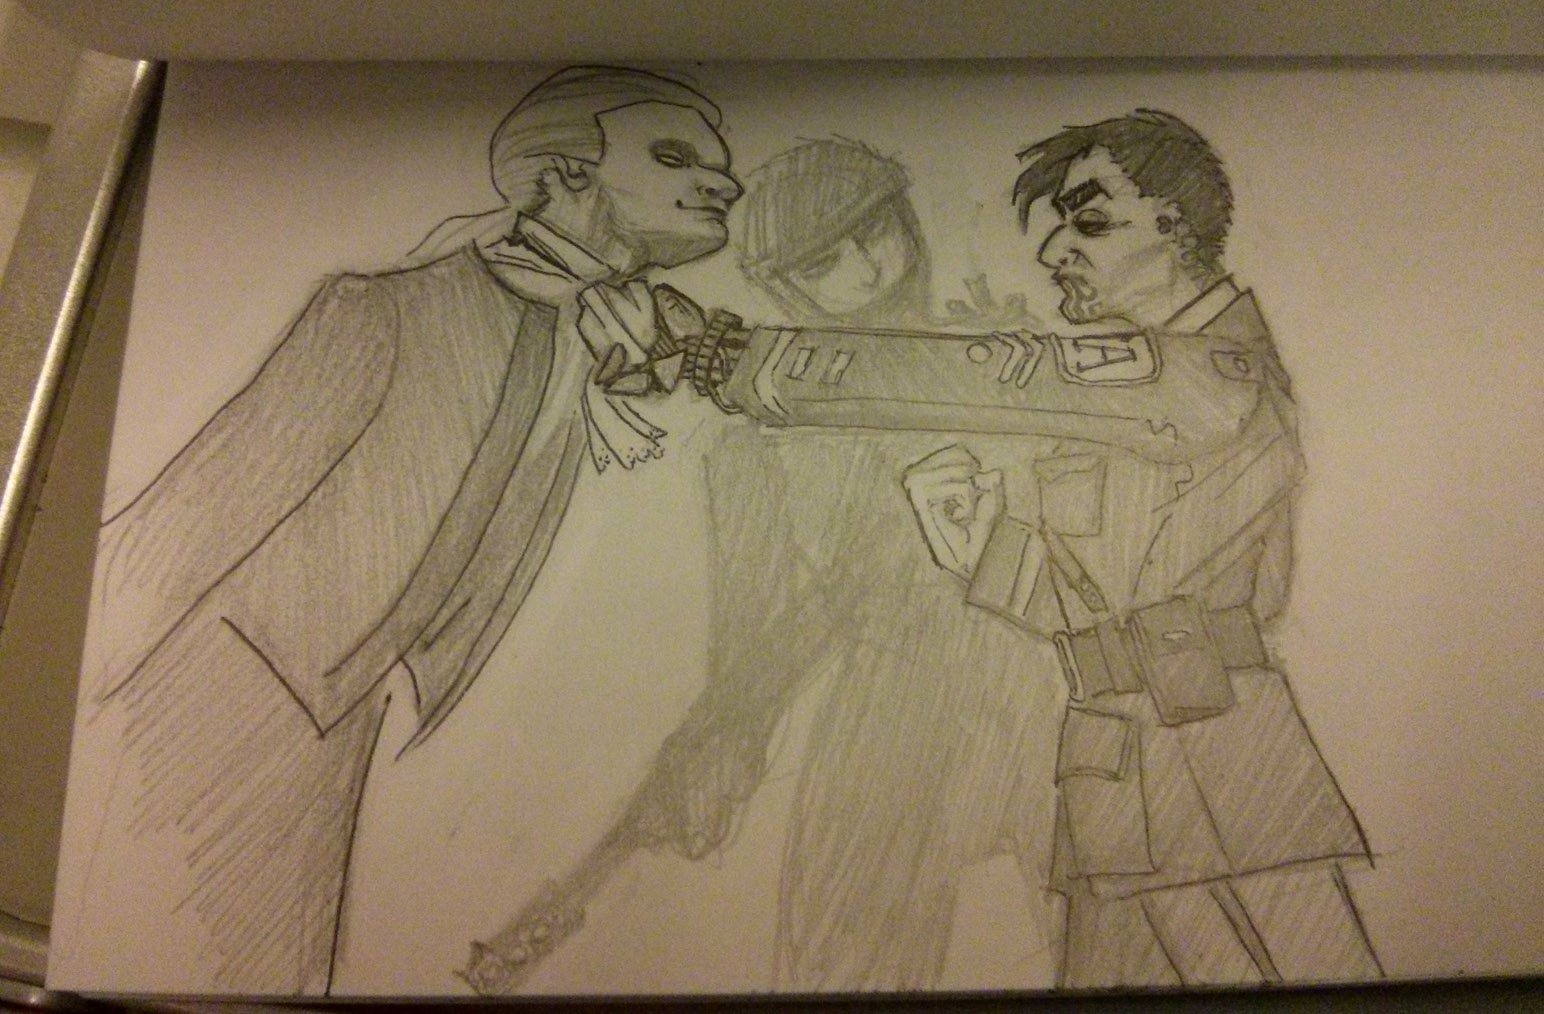
\includegraphics[width=85mm]{img/ch27_diplomatic.jpg}
\end{center}

%\vspace{\fill}

\begin{flushright}
\textsubscript{last edited by \textbf{Rebecca S.} @ 05/29/15 10:57pm}
% Exported @ 08/24/15 3:40pm
\end{flushright}
}




